% Diagrama de flujo del programa TC3 (Nivel 2): lector ADC de potenciometro
% mostrado en display de 7 segmentos, con promedio + histeresis.
% Seminario de Sistemas Embebidos (I7267) - Dr. Ruben Estrada, CUCEI-UDG.
% Compilar: pdflatex diagrama-flujo-tc3.tex  -> PDF recortado (standalone).
\documentclass[border=10pt]{standalone}
\usepackage[T1]{fontenc}
\usepackage[utf8]{inputenc}
\usepackage{lmodern}
\usepackage{xcolor}
\usepackage{tikz}
\usetikzlibrary{shapes.geometric, shapes.misc, arrows.meta, positioning}

\definecolor{optosignal}{HTML}{2A5CAA}
\definecolor{optoemit}{HTML}{C9601F}
\definecolor{optoalert}{HTML}{B23A34}
\definecolor{optodetect}{HTML}{6B4C9A}
\definecolor{optoconfirm}{HTML}{3E7C59}

\tikzset{
  fcstart/.style={rounded rectangle, draw, thick, fill=optoconfirm!18,
    minimum width=2.2cm, minimum height=0.8cm, align=center, font=\footnotesize\bfseries},
  fcproc/.style={rectangle, draw, thick, fill=optodetect!10, rounded corners=2pt,
    minimum width=3.4cm, minimum height=0.8cm, align=center, font=\footnotesize},
  fcio/.style={trapezium, trapezium left angle=70, trapezium right angle=110, draw, thick,
    fill=optoemit!16, minimum width=2.6cm, minimum height=0.7cm, align=center, font=\footnotesize},
  fcdec/.style={diamond, draw, thick, fill=optoalert!14, aspect=2.4, inner sep=1pt,
    align=center, font=\scriptsize},
  fcflecha/.style={-{Triangle[length=2.4mm,width=2.4mm]}, thick},
  fcet/.style={font=\scriptsize\bfseries, inner sep=1.5pt},
}

\begin{document}
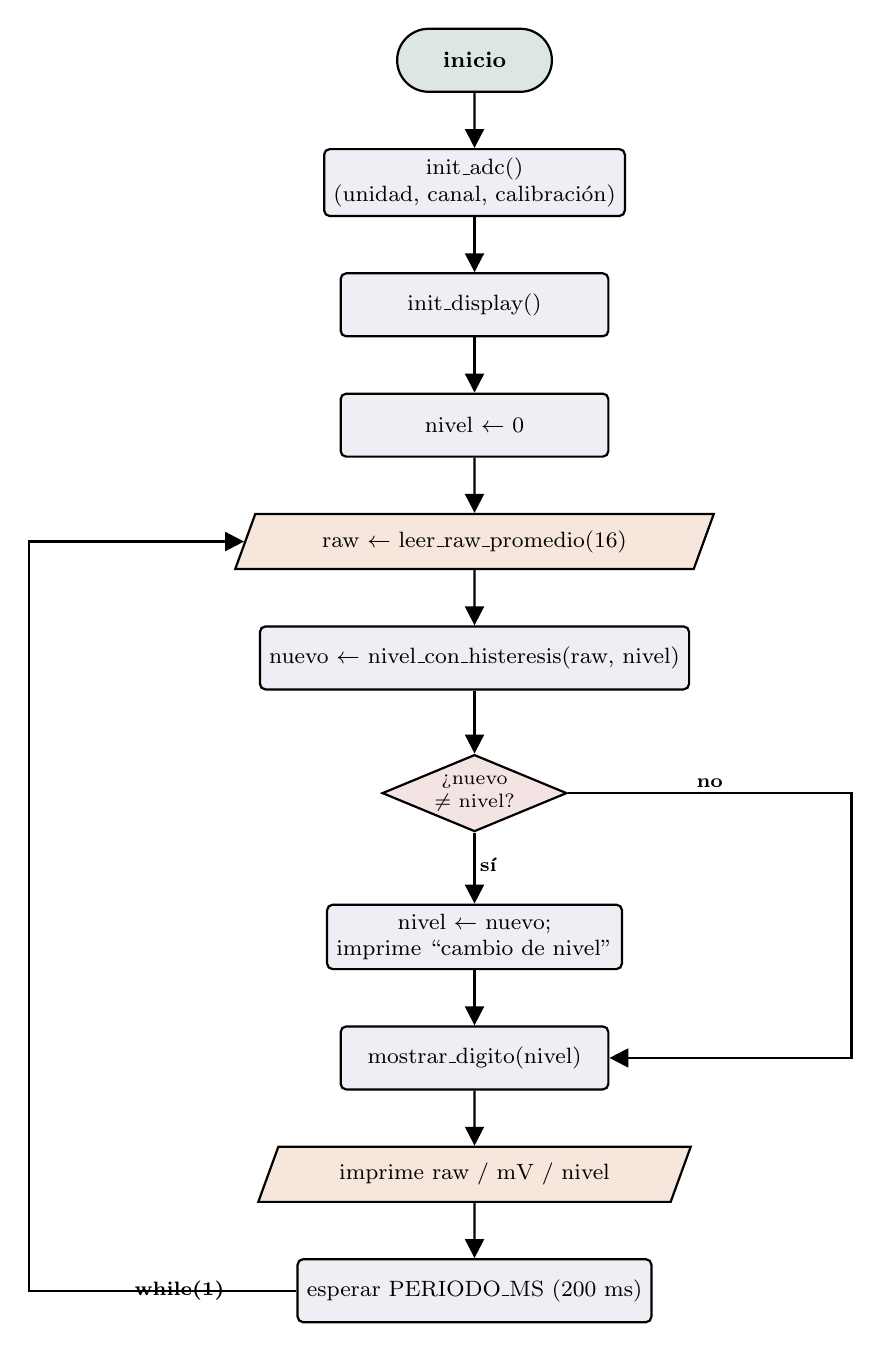
\begin{tikzpicture}[node distance=7mm and 12mm]
  \node[fcstart] (ini) {inicio};
  \node[fcproc, below=of ini] (adc)  {init\_adc()\\(unidad, canal, calibración)};
  \node[fcproc, below=of adc] (disp) {init\_display()};
  \node[fcproc, below=of disp] (n0)  {nivel $\leftarrow$ 0};
  \node[fcio,   below=of n0]  (leer) {raw $\leftarrow$ leer\_raw\_promedio(16)};
  \node[fcproc, below=of leer](hist) {nuevo $\leftarrow$ nivel\_con\_histeresis(raw, nivel)};
  \node[fcdec,  below=8mm of hist](dec) {¿nuevo\\$\neq$ nivel?};
  \node[fcproc, below=9mm of dec] (upd) {nivel $\leftarrow$ nuevo;\\imprime ``cambio de nivel''};
  \node[fcproc, below=of upd] (mos) {mostrar\_digito(nivel)};
  \node[fcio,   below=of mos] (imp) {imprime raw / mV / nivel};
  \node[fcproc, below=of imp] (esp) {esperar PERIODO\_MS (200 ms)};

  \draw[fcflecha] (ini)--(adc);
  \draw[fcflecha] (adc)--(disp);
  \draw[fcflecha] (disp)--(n0);
  \draw[fcflecha] (n0)--(leer);
  \draw[fcflecha] (leer)--(hist);
  \draw[fcflecha] (hist)--(dec);
  \draw[fcflecha] (dec)--(upd) node[fcet, pos=0.45, right]{sí};
  \draw[fcflecha] (upd)--(mos);
  % rama "no": salta la actualizacion, va directo a mostrar
  \draw[fcflecha] (dec.east) -- ++(3.6,0) node[fcet, pos=0.5, above]{no} |- (mos.east);
  \draw[fcflecha] (mos)--(imp);
  \draw[fcflecha] (imp)--(esp);
  % lazo del while(1): de esperar de vuelta a leer (por la izquierda)
  \draw[fcflecha] (esp.west) -- ++(-3.4,0) node[fcet, pos=0.25, left]{while(1)} |- (leer.west);
\end{tikzpicture}
\end{document}
